% Number 540
% UFPM Vectors Algebra Units CAPMA CVPMA
% Wagon rolling down hill
% KO/JG

% Watermark
\AddToShipoutPicture*{\BackgroundPic}

\addtocounter {ProbNum} {1}

%\begin{floatingfigure}[r]{.45\textwidth}
%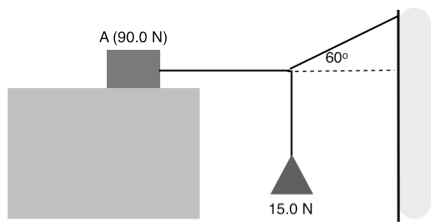
\includegraphics[scale=.6]{/Users/jgates/desktop/latex/pics/static1}
%\end{floatingfigure}
 
{\bf \Large{\arabic{ProbNum}}} A wagon with two boxes of gold (total mass 300 kg) is cut loose from the horses by an outlaw when the wagon is at rest 50 m up a 6 degree slope. The outlaw plans to have the wagon roll down the slope and across the level ground, and then fall into a canyon where his confederates wait. 

\bigskip
Find the speed of the wagon when it reaches the flat ground. Note that it starts from rest at the top of the incline and that the wagon rolls with negligible friction.

\vfill

\vfill
If another bandit standing at the end of the slope requires twenty seconds to grab the gold, how far must the edge of the cliff be from the end of the slope, in order to make this double-heist successful?

%\hfill 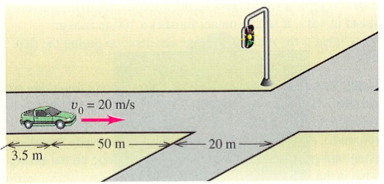
\includegraphics[scale=.85]{/Users/jgates/desktop/latex/pics/redlight.png}


\vfill
\newpage
